\documentclass[UTF8,fontset=none,11pt]{ctexart}
\usepackage[a4paper,margin=2.05cm]{geometry}
\usepackage{amsmath,amssymb}
\usepackage{enumitem}
\usepackage[table]{xcolor}
\usepackage{booktabs}
\usepackage{array}
\usepackage{longtable}
\usepackage{tikz}
\usepackage{graphicx}
\usepackage{hyperref}
\usetikzlibrary{positioning,arrows.meta,shapes.geometric,fit,backgrounds,calc}

\setCJKmainfont[AutoFakeSlant=0.18]{PingFang SC}
\setCJKsansfont[AutoFakeSlant=0.18]{PingFang SC}
\setCJKmonofont[AutoFakeSlant=0.18]{PingFang SC}

\hypersetup{
  colorlinks=true,
  linkcolor=blue!55!black,
  urlcolor=blue!55!black,
  citecolor=blue!55!black,
  pdftitle={RE 到 NFA 到 DFA 到最小化 DFA 学习笔记},
  pdfauthor={Trae AI}
}

\setlength{\parindent}{0pt}
\setlength{\parskip}{0.55em}
\setlist[itemize]{leftmargin=1.8em,itemsep=0.22em,topsep=0.25em}
\setlist[enumerate]{leftmargin=2.0em,itemsep=0.28em,topsep=0.3em}
\renewcommand{\arraystretch}{1.18}
\setlength{\emergencystretch}{3em}
\sloppy

\definecolor{defrule}{RGB}{25,92,140}
\definecolor{noterule}{RGB}{120,80,15}
\definecolor{warnrule}{RGB}{160,50,45}
\definecolor{softblue}{RGB}{235,246,255}
\definecolor{softyellow}{RGB}{255,249,230}
\definecolor{graytext}{RGB}{95,95,95}
\newcolumntype{L}[1]{>{\raggedright\arraybackslash}p{#1}}

\newenvironment{defbox}[1][]{%
  \par\medskip\noindent{\color{defrule}\rule{\linewidth}{1.1pt}}\par\nopagebreak
  \noindent{\bfseries\color{defrule}#1}\par\nopagebreak\smallskip}%
  {\par\nopagebreak\smallskip\noindent{\color{defrule}\rule{\linewidth}{0.4pt}}\par\medskip}
\newenvironment{notebox}[1][]{%
  \par\medskip\noindent{\color{noterule}\rule{\linewidth}{1.1pt}}\par\nopagebreak
  \noindent{\bfseries\color{noterule}#1}\par\nopagebreak\smallskip}%
  {\par\nopagebreak\smallskip\noindent{\color{noterule}\rule{\linewidth}{0.4pt}}\par\medskip}
\newenvironment{warnbox}[1][]{%
  \par\medskip\noindent{\color{warnrule}\rule{\linewidth}{1.1pt}}\par\nopagebreak
  \noindent{\bfseries\color{warnrule}#1}\par\nopagebreak\smallskip}%
  {\par\nopagebreak\smallskip\noindent{\color{warnrule}\rule{\linewidth}{0.4pt}}\par\medskip}

\newcommand{\RE}{\ensuremath{\mathrm{RE}}}
\newcommand{\NFA}{\ensuremath{\mathrm{NFA}}}
\newcommand{\DFA}{\ensuremath{\mathrm{DFA}}}
\newcommand{\eps}{\varepsilon}
\newcommand{\move}{\operatorname{move}}
\newcommand{\eclose}{\operatorname{\epsilon\text{-}closure}}

\tikzset{
  flow/.style={rectangle,rounded corners,draw=defrule,thick,align=center,minimum width=2.8cm,minimum height=0.9cm,fill=softblue},
  smallflow/.style={rectangle,rounded corners,draw=defrule,align=center,minimum width=2.3cm,minimum height=0.75cm,fill=softblue},
  state/.style={circle,draw=black,thick,minimum size=7mm,inner sep=0pt},
  accstate/.style={circle,draw=black,thick,double,minimum size=7mm,inner sep=0pt},
  edge/.style={-{Stealth[length=2.2mm]},thick},
  epsedge/.style={-{Stealth[length=2.2mm]},thick,dashed}
}

\title{\bfseries 从正规表达式到最小 DFA\\词法分析自动机转换完整学习笔记}
\author{RE \(\rightarrow\) Thompson NFA \(\rightarrow\) Subset DFA \(\rightarrow\) Minimized DFA}
\date{\today}

\begin{document}
\maketitle
\tableofcontents
\newpage

\section*{阅读导引}
\addcontentsline{toc}{section}{阅读导引}

词法分析器的核心任务是把源代码字符流切分为 token。一个常见的工程路径是：用正规表达式描述 token 模式，把正规表达式机械地转成 NFA，再把 NFA 转成 DFA，最后最小化 DFA 并生成高效识别代码。

\begin{center}
\resizebox{\linewidth}{!}{
\begin{tikzpicture}[node distance=1.25cm]
  \node[flow] (re) {正规表达式\\Regular Expression};
  \node[flow,right=of re] (nfa) {Thompson 构造\\NFA};
  \node[flow,right=of nfa] (dfa) {子集构造\\DFA};
  \node[flow,right=of dfa] (min) {DFA 最小化\\Minimized DFA};
  \node[flow,right=of min] (lex) {词法分析器\\Lexer};
  \draw[edge] (re) -- (nfa);
  \draw[edge] (nfa) -- (dfa);
  \draw[edge] (dfa) -- (min);
  \draw[edge] (min) -- (lex);
\end{tikzpicture}
}
\end{center}

\begin{notebox}[贯穿示例]
本文使用正规表达式
\[
R=(a|b)^*abb
\]
作为完整示例。它表示所有以 \texttt{abb} 结尾、前面可以有任意个 \texttt{a} 或 \texttt{b} 的字符串，例如 \texttt{abb}、\texttt{aabb}、\texttt{bababb}。
\end{notebox}

\section{基础概念}

\subsection{正规表达式}

\begin{defbox}[正规表达式]
正规表达式是一种描述正规语言的代数记号。它用有限规则描述一类字符串集合，是词法规则最常见的表示方式。
\end{defbox}

常见操作：

\begin{longtable}{L{0.18\linewidth}L{0.28\linewidth}L{0.44\linewidth}}
\toprule
符号 & 名称 & 含义 \\
\midrule
\(a\) & 字符 & 只匹配字符 \(a\) \\
\(\eps\) & 空串 & 匹配长度为 0 的字符串 \\
\(\emptyset\) & 空集 & 不匹配任何字符串 \\
\(r|s\) & 并 / 选择 & 匹配 \(r\) 或 \(s\) \\
\(rs\) & 连接 & 先匹配 \(r\)，再匹配 \(s\) \\
\(r^*\) & Kleene 闭包 & 匹配 0 次或多次 \(r\) \\
\(r^+\) & 正闭包 & 匹配 1 次或多次 \(r\)，可写成 \(rr^*\) \\
\(r?\) & 可选 & 匹配 0 次或 1 次 \(r\)，可写成 \(r|\eps\) \\
\bottomrule
\end{longtable}

运算优先级通常为：闭包最高，连接其次，并最低。因此 \((a|b)^*abb\) 的结构是：
\[
(((a|b)^*)a)b)b.
\]

\subsection{NFA 与 DFA}

\begin{defbox}[NFA]
非确定有限自动机 NFA 是五元组
\[
N=(Q,\Sigma,\delta,q_0,F).
\]
\(Q\) 是状态集合，\(\Sigma\) 是输入字母表，\(\delta\) 是转移函数，\(q_0\) 是初态，\(F\) 是终态集合。NFA 的一个状态在同一输入字符上可以有多个后继，也可以有 \(\eps\) 转移。
\end{defbox}

\begin{defbox}[DFA]
确定有限自动机 DFA 也是五元组
\[
D=(Q,\Sigma,\delta,q_0,F),
\]
但每个状态在每个输入字符上最多有一个确定后继，且没有 \(\eps\) 转移。DFA 运行时只需维护一个当前状态。
\end{defbox}

通俗比较：

\begin{itemize}
  \item NFA 像“同时尝试多条路”。读一个字符后，可能分裂到多个状态。
  \item DFA 像“始终只站在一个确定位置”。每读一个字符，只做一次表查询。
  \item Thompson 算法让 RE 到 NFA 很容易；子集构造把 NFA 的多条可能路径打包成 DFA 的一个状态。
\end{itemize}

\section{Thompson 算法：RE 到 NFA}

\subsection{算法思想}

Thompson 构造把正规表达式看作由小表达式组合而成。每个子表达式都构造一个 NFA 片段，片段有且只有一个入口状态和一个出口状态；然后根据并、连接、闭包等运算把片段拼起来。

\begin{center}
\begin{tikzpicture}[node distance=0.9cm]
  \node[smallflow] (parse) {解析 RE\\得到语法结构};
  \node[smallflow,right=of parse] (base) {为基本项\\建 NFA 片段};
  \node[smallflow,right=of base] (combine) {按运算符\\组合片段};
  \node[smallflow,right=of combine] (out) {得到一个入口\\一个出口的 NFA};
  \draw[edge] (parse) -- (base);
  \draw[edge] (base) -- (combine);
  \draw[edge] (combine) -- (out);
\end{tikzpicture}
\end{center}

\subsection{基本构造规则}

\begin{center}
\resizebox{\linewidth}{!}{
\begin{tikzpicture}[node distance=1.1cm]
  \node[align=center] at (0,1.6) {字符 \(a\)};
  \node[state] (a1) at (-0.9,0.7) {};
  \node[state] (a2) at (0.9,0.7) {};
  \draw[edge] (a1) -- node[above]{\(a\)} (a2);

  \node[align=center] at (4,1.6) {连接 \(rs\)};
  \node[state] (c1) at (2.5,0.7) {};
  \node[state] (c2) at (3.7,0.7) {};
  \node[state] (c3) at (5.0,0.7) {};
  \draw[edge] (c1) -- node[above]{\(r\)} (c2);
  \draw[epsedge] (c2) -- node[above]{\(\eps\)} (c3);
  \node[state] (c4) at (6.2,0.7) {};
  \draw[edge] (c3) -- node[above]{\(s\)} (c4);

  \node[align=center] at (9.5,1.6) {并 \(r|s\)};
  \node[state] (u0) at (8.0,0.7) {};
  \node[state] (u1) at (9.2,1.25) {};
  \node[state] (u2) at (10.5,1.25) {};
  \node[state] (u3) at (9.2,0.15) {};
  \node[state] (u4) at (10.5,0.15) {};
  \node[state] (u5) at (11.7,0.7) {};
  \draw[epsedge] (u0) -- (u1);
  \draw[epsedge] (u0) -- (u3);
  \draw[edge] (u1) -- node[above]{\(r\)} (u2);
  \draw[edge] (u3) -- node[below]{\(s\)} (u4);
  \draw[epsedge] (u2) -- (u5);
  \draw[epsedge] (u4) -- (u5);

  \node[align=center] at (3.0,-1.0) {闭包 \(r^*\)};
  \node[state] (s0) at (0.6,-2.4) {};
  \node[state] (s1) at (2.0,-2.4) {};
  \node[state] (s2) at (3.5,-2.4) {};
  \node[state] (s3) at (4.9,-2.4) {};
  \draw[epsedge] (s0) -- (s1);
  \draw[epsedge] (s0) to[bend left=25] node[above]{\(\eps\)} (s3);
  \draw[edge] (s1) -- node[above]{\(r\)} (s2);
  \draw[epsedge] (s2) -- (s3);
  \draw[epsedge] (s2) to[bend left=35] node[below]{\(\eps\)} (s1);

  \node[align=center] at (9.2,-1.0) {空串 \(\eps\)};
  \node[state] (e1) at (8.3,-2.4) {};
  \node[state] (e2) at (10.1,-2.4) {};
  \draw[epsedge] (e1) -- node[above]{\(\eps\)} (e2);
\end{tikzpicture}
}
\end{center}

\begin{notebox}[为什么 Thompson 构造好用]
它的每个片段接口统一：一个入口、一个出口。连接只需把前一个出口接到后一个入口；并和闭包只需额外加少量 \(\eps\) 边。因此算法可以按语法树后序遍历线性构造。
\end{notebox}

\subsection{Thompson 算法步骤}

\begin{enumerate}
  \item 给正规表达式补充显式连接符，例如把 \((a|b)^*abb\) 看成 \((a|b)^*\cdot a\cdot b\cdot b\)。
  \item 按优先级或语法树解析表达式。
  \item 后序处理语法树：
  \begin{itemize}
    \item 遇到字符、\(\eps\)、\(\emptyset\)，构造基本片段。
    \item 遇到连接、并、闭包，把子片段按规则组合。
  \end{itemize}
  \item 最终得到一个 NFA，初态为总片段入口，终态为总片段出口。
\end{enumerate}

\subsection{复杂度分析}

设正规表达式长度为 \(m\)。

\begin{itemize}
  \item 状态数：\(O(m)\)。每个基本符号和运算符只引入常数个状态。
  \item 转移数：\(O(m)\)。每个构造规则只加入常数条边。
  \item 构造时间：\(O(m)\)。若已完成词法/语法解析，后序遍历即可线性构造。
  \item 空间复杂度：\(O(m)\)。
\end{itemize}

\section{完整示例：构造 Thompson NFA}

对
\[
R=(a|b)^*abb
\]
构造 Thompson NFA。先构造 \(a|b\)，再加闭包 \((a|b)^*\)，最后依次连接 \(a,b,b\)。

\begin{center}
\resizebox{\linewidth}{!}{
\begin{tikzpicture}[node distance=1.1cm]
  \node[state] (q6) at (0,0) {\(6\)};
  \node[state] (q0) at (1.35,0) {\(0\)};
  \node[state] (q1) at (2.7,1.0) {\(1\)};
  \node[state] (q2) at (4.0,1.0) {\(2\)};
  \node[state] (q3) at (2.7,-1.0) {\(3\)};
  \node[state] (q4) at (4.0,-1.0) {\(4\)};
  \node[state] (q5) at (5.35,0) {\(5\)};
  \node[state] (q7) at (6.75,0) {\(7\)};
  \node[state] (q8) at (8.1,0) {\(8\)};
  \node[state] (q9) at (9.45,0) {\(9\)};
  \node[state] (q10) at (10.8,0) {\(10\)};
  \node[state] (q11) at (12.15,0) {\(11\)};
  \node[state] (q12) at (13.5,0) {\(12\)};
  \node[accstate] (q13) at (14.85,0) {\(13\)};

  \draw[edge] (-0.8,0) -- (q6);
  \draw[epsedge] (q6) -- node[above]{\(\eps\)} (q0);
  \draw[epsedge] (q6) to[bend left=25] node[above]{\(\eps\)} (q7);
  \draw[epsedge] (q0) -- (q1);
  \draw[epsedge] (q0) -- (q3);
  \draw[edge] (q1) -- node[above]{\(a\)} (q2);
  \draw[edge] (q3) -- node[below]{\(b\)} (q4);
  \draw[epsedge] (q2) -- (q5);
  \draw[epsedge] (q4) -- (q5);
  \draw[epsedge] (q5) to[bend left=38] node[below]{\(\eps\)} (q0);
  \draw[epsedge] (q5) -- node[above]{\(\eps\)} (q7);
  \draw[epsedge] (q7) -- node[above]{\(\eps\)} (q8);
  \draw[edge] (q8) -- node[above]{\(a\)} (q9);
  \draw[epsedge] (q9) -- node[above]{\(\eps\)} (q10);
  \draw[edge] (q10) -- node[above]{\(b\)} (q11);
  \draw[epsedge] (q11) -- node[above]{\(\eps\)} (q12);
  \draw[edge] (q12) -- node[above]{\(b\)} (q13);

  \node[draw=noterule,rounded corners,align=left,fill=softyellow] at (7.4,-2.0) {
    初态：\(6\)；终态：\(13\)。\\
    \(6,0,1,2,3,4,5,7\) 负责 \((a|b)^*\)。\\
    后面的 \(8\to9\to10\to11\to12\to13\) 负责后缀 \(abb\)。
  };
\end{tikzpicture}
}
\end{center}

从这张图可以看出，\(\eps\) 边负责“自动选择路径”或“重复/跳过”。例如状态 6 可通过 \(\eps\) 直接到状态 7，表示 \((a|b)^*\) 可以重复 0 次；状态 5 可通过 \(\eps\) 回到状态 0，表示继续重复。

\section{子集构造法：NFA 到 DFA}

\subsection{核心思想}

DFA 运行时只能处在一个状态，而 NFA 可能同时处在多个状态。子集构造法的关键是：把 NFA 的一个状态集合当作 DFA 的一个状态。

\begin{defbox}[epsilon-closure]
\(\eclose(S)\) 表示从状态集合 \(S\) 出发，只沿 \(\eps\) 边能到达的所有状态，包括 \(S\) 本身。
\end{defbox}

\begin{defbox}[move]
\(\move(S,a)\) 表示从状态集合 \(S\) 中任意状态出发，沿字符 \(a\) 边能到达的状态集合。
\end{defbox}

子集构造的转移公式是：
\[
T'=\eclose(\move(T,a)).
\]
其中 \(T\) 是一个 DFA 状态，也就是一组 NFA 状态；\(a\) 是输入字符。

\subsection{算法流程}

\begin{center}
\begin{tikzpicture}[node distance=0.9cm]
  \node[flow] (s0) {起始集合\\\(\eclose(\{q_0\})\)};
  \node[flow,right=of s0] (pick) {取一个尚未\\处理的集合 \(T\)};
  \node[flow,right=of pick] (each) {对每个字符 \(a\)\\计算 \(U=\eclose(\move(T,a))\)};
  \node[flow,right=of each] (new) {若 \(U\) 未出现\\加入 DFA 状态};
  \node[flow,below=of each] (done) {所有集合处理完\\得到 DFA};
  \draw[edge] (s0) -- (pick);
  \draw[edge] (pick) -- (each);
  \draw[edge] (each) -- (new);
  \draw[edge] (new) to[bend left=15] (pick);
  \draw[edge] (each) -- (done);
\end{tikzpicture}
\end{center}

伪代码：

\begin{verbatim}
Dstates = { epsilon-closure({NFA_start}) }
while exists unmarked T in Dstates:
    mark T
    for each input symbol a:
        U = epsilon-closure(move(T, a))
        if U is not in Dstates:
            add U to Dstates
        Dtran[T, a] = U
\end{verbatim}

若某个 DFA 状态集合包含 NFA 终态，则该 DFA 状态就是终态。

\subsection{复杂度分析}

设 NFA 有 \(n\) 个状态，字母表大小为 \(|\Sigma|\)。

\begin{itemize}
  \item 最坏 DFA 状态数：\(2^n\)。因为 NFA 状态集合最多有 \(2^n\) 种。
  \item 转移计算：每个可达子集要对每个输入字符计算一次 move 和 closure。
  \item 朴素实现时间：可写为 \(O(2^n|\Sigma|(n+e))\)，其中 \(e\) 为 NFA 转移数。
  \item 实际情况：词法分析中的正则通常结构简单，可达子集远少于 \(2^n\)，因此工程上可接受。
\end{itemize}

\section{完整示例：子集构造 DFA}

对上一节的 NFA，字母表 \(\Sigma=\{a,b\}\)。从初态 6 开始：

\[
A=\eclose(\{6\})=\{0,1,3,6,7,8\}.
\]

逐步计算得到 DFA 状态：

\begin{longtable}{L{0.10\linewidth}L{0.48\linewidth}L{0.16\linewidth}L{0.16\linewidth}}
\toprule
DFA 状态 & NFA 状态集合 & 输入 \(a\) & 输入 \(b\) \\
\midrule
\(A\) & \(\{0,1,3,6,7,8\}\) & \(B\) & \(C\) \\
\(B\) & \(\{0,1,2,3,5,7,8,9,10\}\) & \(B\) & \(D\) \\
\(C\) & \(\{0,1,3,4,5,7,8\}\) & \(B\) & \(C\) \\
\(D\) & \(\{0,1,3,4,5,7,8,11,12\}\) & \(B\) & \(E\) \\
\(E\) & \(\{0,1,3,4,5,7,8,13\}\) & \(B\) & \(C\) \\
\bottomrule
\end{longtable}

状态 \(E\) 包含 NFA 终态 13，因此 \(E\) 是 DFA 终态。

\begin{center}
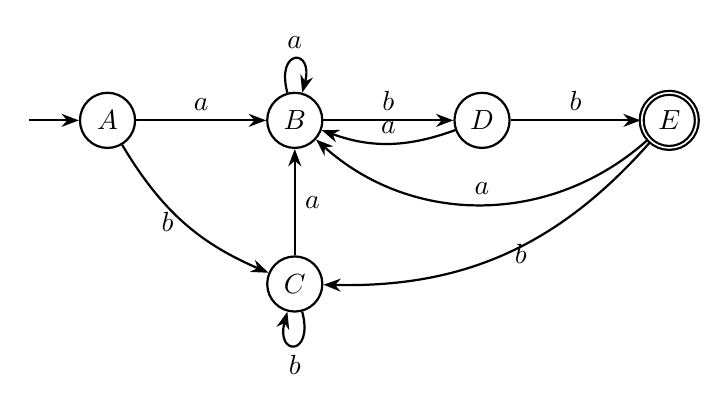
\begin{tikzpicture}[node distance=1.65cm]
  \node[state] (A) {\(A\)};
  \node[state,right=of A] (B) {\(B\)};
  \node[state,right=of B] (D) {\(D\)};
  \node[accstate,right=of D] (E) {\(E\)};
  \node[state,below=1.35cm of B] (C) {\(C\)};

  \draw[edge] (-1.0,0) -- (A);
  \draw[edge] (A) -- node[above]{\(a\)} (B);
  \draw[edge] (A) to[bend right=18] node[left]{\(b\)} (C);
  \draw[edge] (B) to[loop above] node{\(a\)} (B);
  \draw[edge] (B) -- node[above]{\(b\)} (D);
  \draw[edge] (C) -- node[right]{\(a\)} (B);
  \draw[edge] (C) to[loop below] node{\(b\)} (C);
  \draw[edge] (D) to[bend left=20] node[above]{\(a\)} (B);
  \draw[edge] (D) -- node[above]{\(b\)} (E);
  \draw[edge] (E) to[bend left=42] node[above]{\(a\)} (B);
  \draw[edge] (E) to[bend left=25] node[right]{\(b\)} (C);
\end{tikzpicture}
\end{center}

这个 DFA 已经没有 \(\eps\) 转移，也不会在同一字符上分裂到多个状态。但它还不是最小的，因为 \(A\) 和 \(C\) 行为完全相同。

\section{DFA 最小化}

\subsection{为什么要最小化}

DFA 的执行速度主要由“当前状态 + 输入字符”的转移表查询决定；状态越少，表越小，生成的词法分析器通常越紧凑。DFA 最小化就是把识别同一语言且行为不可区分的状态合并。

\begin{defbox}[等价状态]
两个 DFA 状态 \(p,q\) 等价，是指从 \(p\) 和 \(q\) 出发，读任意后缀字符串 \(w\)，最终接受/拒绝结果都相同。这样的状态可以合并。
\end{defbox}

\subsection{划分细化算法}

最常用的直观算法是 partition refinement：

\begin{enumerate}
  \item 初始划分为两组：终态集合 \(F\) 与非终态集合 \(Q-F\)。
  \item 对每个分组，检查其中状态在每个输入字符上的转移目标属于哪个分组。
  \item 若同一组中存在状态在某字符上跳到不同分组，则拆分该组。
  \item 重复细化，直到所有分组都不能再拆。
  \item 每个分组合并为最小 DFA 的一个状态。
\end{enumerate}

\begin{center}
\resizebox{\linewidth}{!}{
\begin{tikzpicture}[node distance=1.0cm]
  \node[flow] (init) {初始划分\\终态 / 非终态};
  \node[flow,right=of init] (check) {检查每组中\\转移目标分组};
  \node[flow,right=of check] (split) {若行为不同\\拆分分组};
  \node[flow,right=of split] (fix) {直到无法再拆\\得到等价类};
  \node[flow,right=of fix] (merge) {每个等价类\\合并成状态};
  \draw[edge] (init) -- (check);
  \draw[edge] (check) -- (split);
  \draw[edge] (split) -- (fix);
  \draw[edge] (fix) -- (merge);
  \draw[edge] (split) to[bend right=32] node[below]{继续检查} (check);
\end{tikzpicture}
}
\end{center}

\subsection{复杂度分析}

设 DFA 有 \(k\) 个状态，字母表大小为 \(|\Sigma|\)。

\begin{itemize}
  \item 朴素表填法：通常为 \(O(k^2|\Sigma|)\)。
  \item 普通划分细化：实现不同，常见朴素版本可到 \(O(k^2|\Sigma|)\)。
  \item Hopcroft 算法：经典最优量级之一，为 \(O(|\Sigma|k\log k)\)。
  \item 空间复杂度：至少需要保存转移表 \(O(k|\Sigma|)\)，以及划分或标记信息。
\end{itemize}

\section{完整示例：DFA 最小化}

当前 DFA 状态为 \(A,B,C,D,E\)，其中 \(E\) 是终态。

初始划分：
\[
P_0=\{\{E\},\{A,B,C,D\}\}.
\]

检查非终态组 \(\{A,B,C,D\}\)：

\begin{longtable}{L{0.13\linewidth}L{0.18\linewidth}L{0.18\linewidth}L{0.38\linewidth}}
\toprule
状态 & 输入 \(a\) 的目标组 & 输入 \(b\) 的目标组 & 结论 \\
\midrule
\(A\) & 非终态组 & 非终态组 & 与 \(C\) 相同行为 \\
\(B\) & 非终态组 & 非终态组 & 暂时可与 \(A,C\) 同组，但后续需再细分 \\
\(C\) & 非终态组 & 非终态组 & 与 \(A\) 相同行为 \\
\(D\) & 非终态组 & 终态组 & 必须单独分出 \\
\bottomrule
\end{longtable}

第一次细分：
\[
P_1=\{\{E\},\{D\},\{A,B,C\}\}.
\]

继续检查 \(\{A,B,C\}\)：

\begin{itemize}
  \item \(A\) 在 \(a\) 上到 \(B\)，在 \(b\) 上到 \(C\)，都在 \(\{A,B,C\}\)。
  \item \(C\) 在 \(a\) 上到 \(B\)，在 \(b\) 上到 \(C\)，都在 \(\{A,B,C\}\)。
  \item \(B\) 在 \(a\) 上到 \(B\)，在 \(b\) 上到 \(D\)，而 \(D\) 已经是单独分组。
\end{itemize}

因此：
\[
P_2=\{\{E\},\{D\},\{B\},\{A,C\}\}.
\]

此时无法继续细分。合并 \(A\) 和 \(C\)，得到最小 DFA：

\begin{longtable}{L{0.17\linewidth}L{0.23\linewidth}L{0.23\linewidth}L{0.25\linewidth}}
\toprule
最小状态 & 来源 & 输入 \(a\) & 输入 \(b\) \\
\midrule
\(S_0\) & \(\{A,C\}\) & \(S_1\) & \(S_0\) \\
\(S_1\) & \(\{B\}\) & \(S_1\) & \(S_2\) \\
\(S_2\) & \(\{D\}\) & \(S_1\) & \(S_3\) \\
\(S_3\) & \(\{E\}\) & \(S_1\) & \(S_0\) \\
\bottomrule
\end{longtable}

\begin{center}
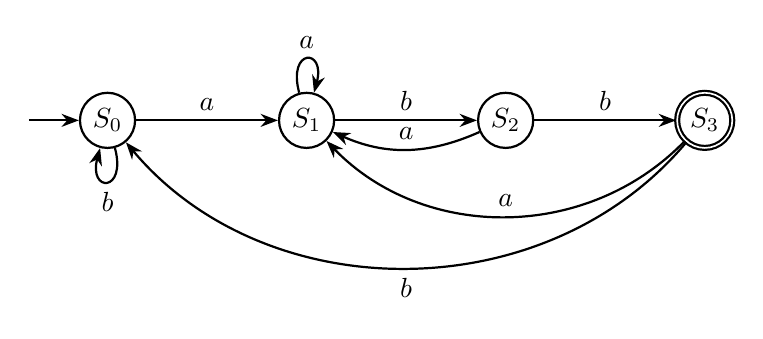
\begin{tikzpicture}[node distance=1.8cm]
  \node[state] (S0) {\(S_0\)};
  \node[state,right=of S0] (S1) {\(S_1\)};
  \node[state,right=of S1] (S2) {\(S_2\)};
  \node[accstate,right=of S2] (S3) {\(S_3\)};

  \draw[edge] (-1.0,0) -- (S0);
  \draw[edge] (S0) -- node[above]{\(a\)} (S1);
  \draw[edge] (S0) to[loop below] node{\(b\)} (S0);
  \draw[edge] (S1) to[loop above] node{\(a\)} (S1);
  \draw[edge] (S1) -- node[above]{\(b\)} (S2);
  \draw[edge] (S2) to[bend left=24] node[above]{\(a\)} (S1);
  \draw[edge] (S2) -- node[above]{\(b\)} (S3);
  \draw[edge] (S3) to[bend left=46] node[above]{\(a\)} (S1);
  \draw[edge] (S3) to[bend left=50] node[below]{\(b\)} (S0);
\end{tikzpicture}
\end{center}

这个最小 DFA 的含义非常直观：

\begin{itemize}
  \item \(S_0\)：当前尚未匹配到有用后缀，或当前后缀相当于“无前缀匹配”。
  \item \(S_1\)：当前最长匹配后缀是 \(a\)。
  \item \(S_2\)：当前最长匹配后缀是 \(ab\)。
  \item \(S_3\)：当前最长匹配后缀是 \(abb\)，接受。
\end{itemize}

\section{工程实现提示}

\subsection{从多个 token 规则构造词法分析器}

真实词法分析器通常不只处理一个正规表达式，而是处理多条 token 规则：

\[
R_1,\ R_2,\ \ldots,\ R_n.
\]

常见做法：

\begin{enumerate}
  \item 分别为每个 \(R_i\) 构造 Thompson NFA。
  \item 新建一个总初态，用 \(\eps\) 边连到每个规则 NFA 的初态。
  \item 每个规则的终态标注 token 类型和优先级。
  \item 子集构造后，若一个 DFA 状态包含多个 NFA 终态，按优先级选 token。
  \item 扫描输入时采用最长匹配原则：不断前进，记录最近一次到达接受状态的位置和 token。
\end{enumerate}

\subsection{常见易错点}

\begin{itemize}
  \item 忘记在子集构造中每一步都做 \(\eps\)-closure。
  \item 把 NFA 的“多个可能状态”误当作 DFA 的“多个当前状态”。DFA 状态本身就是一个集合。
  \item 最小化前没有删除不可达状态。严格流程通常先删除从初态不可达的状态，再做最小化。
  \item 只用“是否终态”判断等价状态。终态/非终态只是初始划分，后续还要看所有字符的转移行为。
  \item 在真实 lexer 中忽略最长匹配和规则优先级。
\end{itemize}

\section{练习题与解答}

\subsection*{题 1：为什么 Thompson NFA 通常有很多 epsilon 转移？}

\textbf{解答：} 因为 Thompson 构造要保持“每个片段一个入口、一个出口”的统一接口。并、闭包、连接都通过 \(\eps\) 边把片段组合起来。这样构造规则简单，代价是 NFA 中出现大量 \(\eps\) 转移，后续需要用 \(\eps\)-closure 处理。

\subsection*{题 2：对子集构造，为什么 DFA 状态是 NFA 状态集合？}

\textbf{解答：} NFA 在读入一个前缀后，可能同时处在多个状态。为了用 DFA 模拟 NFA，必须把这些“所有可能状态”整体记录下来。这个集合就是 DFA 的一个状态。

\subsection*{题 3：在本文示例中，初始 DFA 状态 A 是什么？}

\textbf{解答：}
\[
A=\eclose(\{6\})=\{0,1,3,6,7,8\}.
\]
它包含初态 6 以及只沿 \(\eps\) 边能到达的所有状态。

\subsection*{题 4：为什么状态 E 是 DFA 接受状态？}

\textbf{解答：} 因为
\[
E=\{0,1,3,4,5,7,8,13\}
\]
包含 Thompson NFA 的终态 13。子集构造中，只要某个 DFA 状态集合包含任一 NFA 终态，该 DFA 状态就是接受状态。

\subsection*{题 5：为什么示例 DFA 中 A 和 C 可以合并？}

\textbf{解答：} A 和 C 都不是终态，并且它们对每个输入字符的行为完全相同：
\[
A \xrightarrow{a} B,\quad A \xrightarrow{b} C,
\]
\[
C \xrightarrow{a} B,\quad C \xrightarrow{b} C.
\]
读任意后缀时，从 A 和 C 出发的接受/拒绝结果都相同，因此二者等价。

\subsection*{题 6：最小 DFA 有几个状态？分别表示什么？}

\textbf{解答：} 对 \((a|b)^*abb\)，最小 DFA 有 4 个状态：

\begin{itemize}
  \item \(S_0\)：当前后缀没有匹配到模式前缀。
  \item \(S_1\)：当前后缀是 \(a\)。
  \item \(S_2\)：当前后缀是 \(ab\)。
  \item \(S_3\)：当前后缀是 \(abb\)，接受。
\end{itemize}

\subsection*{题 7：如果输入串是 \texttt{bababb}，最小 DFA 如何运行？}

\textbf{解答：}
\[
S_0 \xrightarrow{b} S_0 \xrightarrow{a} S_1 \xrightarrow{b} S_2 \xrightarrow{a} S_1 \xrightarrow{b} S_2 \xrightarrow{b} S_3.
\]
最终到达接受状态 \(S_3\)，所以 \texttt{bababb} 被接受。

\subsection*{题 8：如果输入串是 \texttt{ababa}，是否接受？}

\textbf{解答：}
\[
S_0 \xrightarrow{a} S_1 \xrightarrow{b} S_2 \xrightarrow{a} S_1 \xrightarrow{b} S_2 \xrightarrow{a} S_1.
\]
最终在 \(S_1\)，不是接受状态，因此不接受。\texttt{ababa} 不以 \texttt{abb} 结尾。

\subsection*{题 9：三种算法的最坏复杂度分别是什么？}

\textbf{解答：} Thompson 构造对 RE 长度 \(m\) 是 \(O(m)\)。子集构造对 NFA 状态数 \(n\) 最坏可产生 \(2^n\) 个 DFA 状态，因此最坏指数级。DFA 最小化若用朴素方法常见为 \(O(k^2|\Sigma|)\)，Hopcroft 算法可达 \(O(|\Sigma|k\log k)\)，其中 \(k\) 是 DFA 状态数。

\section*{复习总结}
\addcontentsline{toc}{section}{复习总结}

完整流程可以浓缩为：

\begin{enumerate}
  \item RE 描述语言规则。
  \item Thompson 算法把 RE 机械地构造成带 \(\eps\) 转移的 NFA。
  \item 子集构造用 NFA 状态集合模拟 NFA 的所有可能路径，得到 DFA。
  \item DFA 最小化合并等价状态，得到更小的识别器。
  \item 词法分析器基于最小 DFA 做高速扫描，并在多 token 情况下结合最长匹配和规则优先级。
\end{enumerate}

理解这条链路的关键是两句话：Thompson 用 \(\eps\) 边让构造变简单；子集构造用“状态集合”把不确定性变成确定性。

\end{document}
